\documentclass{article}
\usepackage{hyperref}
\usepackage[margin=0.5in]{geometry}
\usepackage{amsmath}
\usepackage{graphicx}
\usepackage[bottom]{footmisc}
\usepackage{lastpage}
\usepackage{fancyhdr}
\usepackage{float}
\usepackage{tabularx}

\graphicspath{ {./assets/} }

\pagestyle{fancy}
\fancyhf{} % clear existing header/footer entries
% Place Page X of Y on the right-hand
% side of the footer
\fancyfoot[R]{Yang \thepage \hspace{1pt} of \pageref{LastPage}}
\renewcommand{\headrulewidth}{0pt}

\title{PHYSIOL 578: HW 3.1\footnotetext{U-M GPT was used to help draft and refine the answers.}}
\author{Jack Yang \\ \href{mailto:yhyunjoo@umich.edu}{yhyunjoo@umich.edu}}

\begin{document}
\maketitle
\thispagestyle{fancy}

\section{
    You are studying a synaptic connection between two neurons – A and B – in cell
culture . Describe an experiment you could do to determine whether the synapse between
Neurons A and B is electrical or chemical in nature. How would the results point to one
synapse type over the other? (3 points)
}

You could record the timing of the activity of the two neurons.
If stimulation of one neuron immediately results in the activity of the other neuron without delay,
the synapse is likely electrical.
Also, you could test for directionality.
If stimulation of one neuron causes activity in the other,
but not vice versa, this points to chemical synapse.

\section{
    You are studying a novel synaptic protein GRND and are interested in whether it
alters presynaptic or postsynaptic function. To examine this question, you make hippocampal
slices from either wild-type (+/+; control) or GRND knockout (-/-) mice. Using field-potential
recordings in hippocampal area CA1, you stimulate Schaffer collateral fibers using paired
stimuli spaced by a variable inter-stimulus interval. The concentration of Ca2+ in your aCSF is
1 mM. You acquire the data shown below.
}



\subsection{
    Does this data suggest that GRND regulates
synaptic function and if so, is the effect likely
presynaptic or postsynaptic? Justify your answer.
(2 points)
}

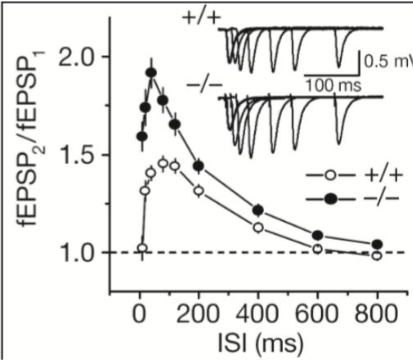
\includegraphics{fig1.png}

Yes, the difference in fEPSP2/fEPSP1 between the control and knockout
indicates that GRND indeed regulates synaptic function.
It seems to affect presynaptic plasticity as lack of GRND leads to higher paired-pulse ratio (and higher facilitation),
indicating lower release probability (Pr).

\subsection{
    Recording just from GRND knockout slices, if you
raised the concentration of Ca2+ in your aCSF from 1 to 4 mM, would the results likely further
diverge from what is observed in wild-type slices at 1 mM Ca2+? Or, would the results be
more similar? Explain your prediction. (2 points)
}
The increase in the concentration of calcium ion would likely
lead to higher probability of release which means the first pulse causes more synapses
to release vesicles and depletes the readily releasable pool,
leaving less room for facilitation,
leading to a less divergence from wild-type slices.

\subsection{
    To explore GRND's role further, you switch to
whole-cell voltage-clamp recordings of CA1
neurons and use AMPAR and GABA-A receptor
antagonists to isolate NMDAR-mediated EPSCs
(recorded at -60 mV). You stimulate Schaffer
collateral fibers to evoke single action potentials
in the population of CA3 neurons synapsing onto
the CA1 neuron you are recording from in the
presence of 10 $\mu$M MK-801. MK-801 irreversibly
blocks NMDARs, but only after they open (use-
dependent blocker). You derive the data shown
on the right following repetitive activation of
Schaffer collaterals in the presence of MK-801. The data are normalized to the amplitude of
the NMDAR current on the first stimulation.
\\
\\
Based on these results, what aspect of synaptic transmission is likely altered in the GRND
knockout mice. Explain your answer. (2 points)
}

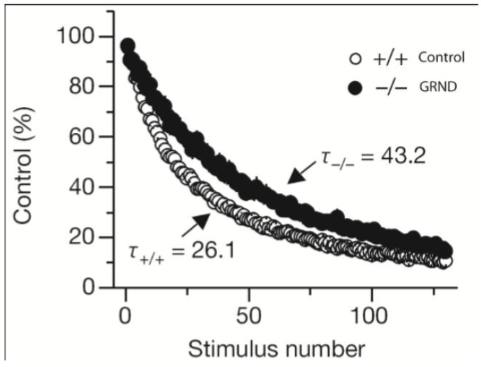
\includegraphics{fig2.png}

The results seem to further support that the release probability is decreased
in the absence of GRND. With lower release probability (consistent with higher facilitation in questions above),
less synapses release vesicles therefore opening the NMDARs less and thus blocking them less.

\subsection{
    Assume your stimulation activates an identical number of CA3 axons in the two genotypes,
would you predict that the first NMDAR EPSC would be smaller, larger, or unaltered in the
GRND knockouts relative to wild-type. Why? (2 points)
}
I would expect the first NMDAR EPSC to be smaller in the GRND knockouts
since synapses are less likely to release vesicles.

\subsection{
    A colleague of yours notes that GRND has a c-terminal SNARE motif, and hypothesizes that
native GRND binds syntaxin1A and prevents it from associating with SNAP25 and
VAMP/synaptobrevin. Do your results support this hypothesis? Do they refute it? Or do they
not provide sufficient information one way or the other? Explain your answer. (2 points)
}
The results seem to refute that GRND prevents syntaxin1A from associating with
SNAP25 and VAMP/synaptobrevin which are essential components for vesicle fusion.
If GRND did indeed prevent the association, we would see an increase in release probability
(decrease in facilitation) in knockout type, but we saw a decrease.

\section{
    You are studying a recently identified PSD protein known as RAM. You
hypothesize that RAM selectively modulates NMDARs without affecting AMPARs. To test this
idea, you have prepared acute hippocampal slices from RAM knockout mice and wild-type
littermate controls. But it is the weekend and you have been inadvertently locked out from the
lab’s chemical inventory, so you do not have access to any pharmaceuticals. Design an
experimental protocol that would allow you to measure the NMDAR component of the EPSC to
compare between wild-type and knockout slices. Briefly explain the rationale. (3 points)
}
Without drugs, I would separate NMDAR and AMPAR currents using their different voltage dependence. In whole-cell recordings from CA1 neurons, I would evoke EPSCs at a negative holding potential, where Mg2+ blocks NMDARs and the current is AMPAR-mediated, and then at a positive holding potential, where the block is relieved and a slow NMDAR component appears. Comparing the NMDAR component relative to the AMPAR component in WT and KO slices would show whether RAM selectively affects NMDARs.

\end{document}